\documentclass[../../main.tex]{subfiles}

\begin{document}
    Wir widmen uns nun der Lebensdauerbestimmung des angeregten Nd:YAG Kristallniveaus $4F_{3/2}$. 

    Hierzu legen wir per Zwischenschaltung eines Funktionsgenerators einen mit $f = 50\,\si{\hertz}$ fluktuierenden Strom an. Dies führt zu Niveaubevölkerung und anschließender Photonenemission, in Form einer Spannung am Oszilloskop messen. Hiebei erhalten wir einen exponentiellen Abfall nach einem Plateau höchster Niveaubevölkerung, wie in Abbildung \ref{fig:2-spontaneEmissionDataT} zu sehen ist. Um eine Zeitskala auf der $x$-Achse zu erzielen, musste die Zeititerationsachse der Messwerte per linearer Funktion $t(z) := 5\cdot 10^{-6}\si{\s}\cdot z - 2.93\cdot 10^{-3}\si{\s}$ umgerechnet werden. Die Unsicherheiten übertragen sich hier theoretisch linear, jedoch sind vom Messgerät in dieser Achse keine solchen angegeben. Ebenfalls sind die gemessenen Spannungswerte unsicherheitsfrei eingelesen worden. 
    \begin{figure}[H]
        \centering
        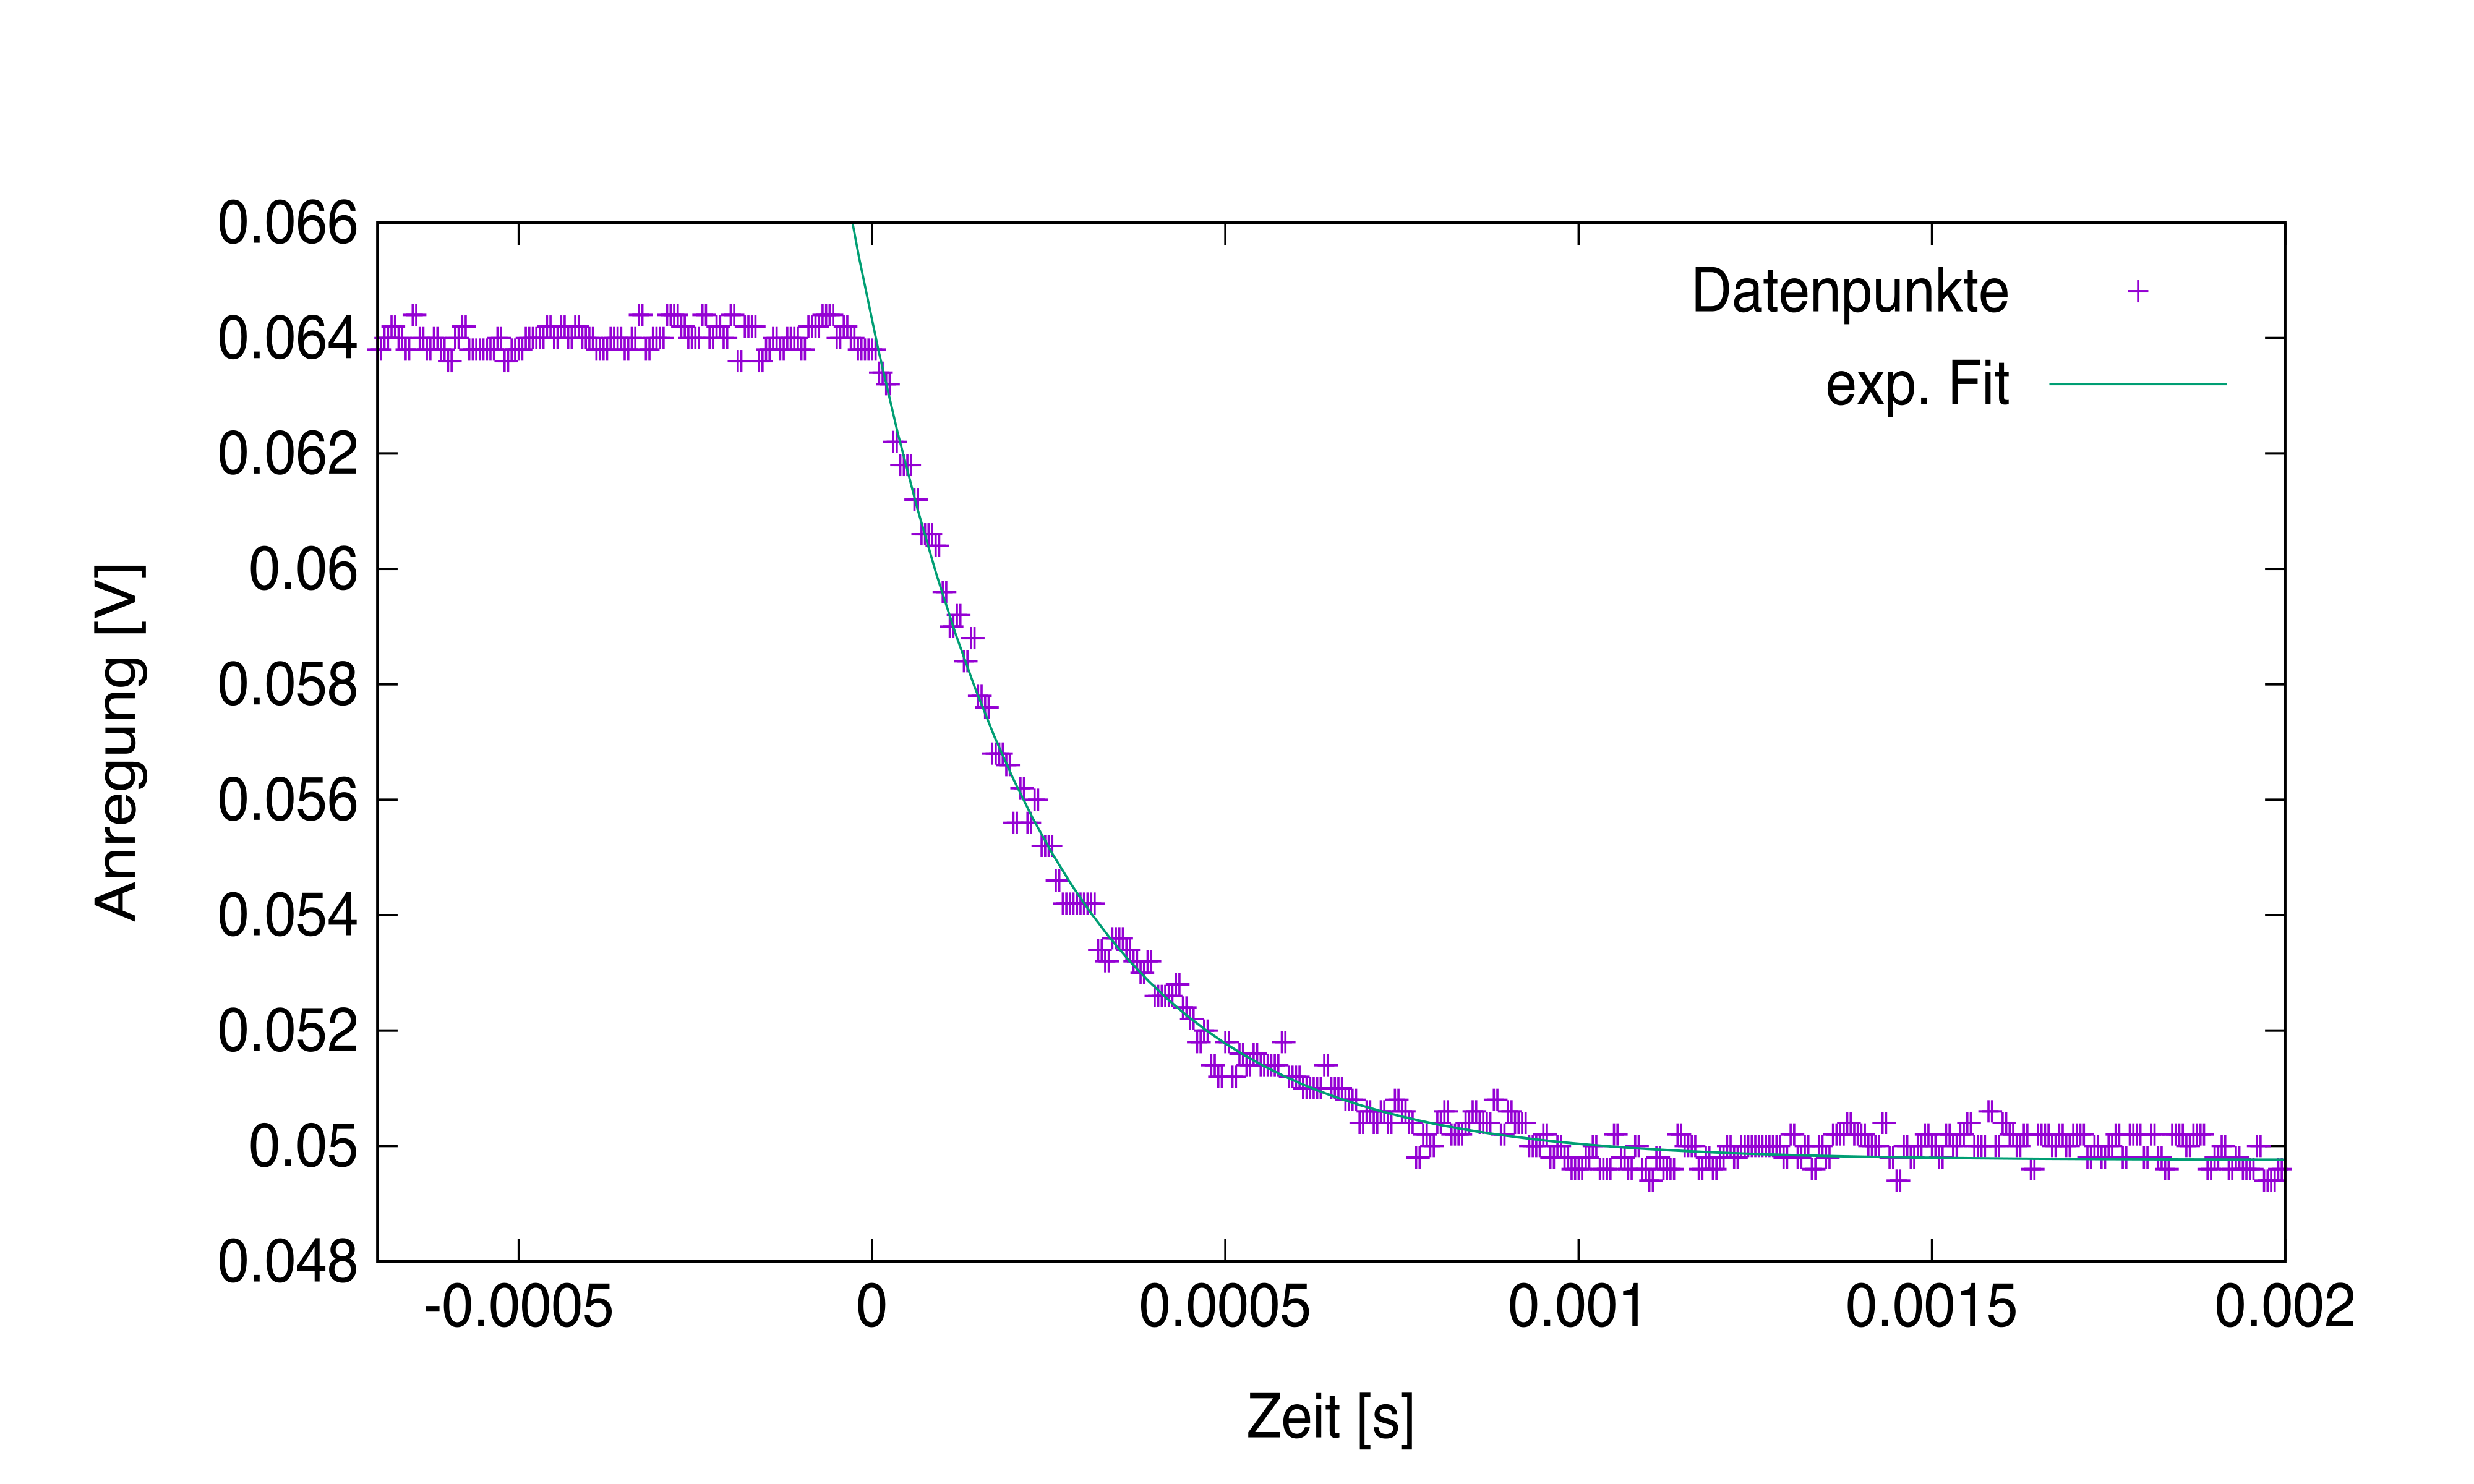
\includegraphics[width=11cm]{../../Bilddateien/2/spontane_emission_data_t.png}
        \caption{Die gemessene Spannung als Funktion der Zeit.}
        \label{fig:2-spontaneEmissionDataT}
    \end{figure}
    Führen wir anhand Abbildung \ref{fig:2:spontaneEmissionDataT} eine exponentiell abfallende Kurvenanpassung der Form 
    \[
        f_{a,\tau,c}(x) := a\cdot \exp(-\frac{x}{\tau}) + c
    \]
    ab dem ersten vom Plateau abfallenden Spannungswert durch, so erhalten wir optisch den in Abbildung \ref{fig:2-spontaneEmissionDataT} dargestellten Fit. Die Parameter $a,\tau,c$ und ihre zugehörigen asymptotischen Standardunsicherheiten $u(a),u(\tau),u(c)$ sind in Tabelle \ref{tab:2-spontaneEmissionDataTExpFit} aufgeführt.
    
    %% ======================== ENTFERNT WEGEN IMPLEMENTIERUNG IN OBIGE ABBILDUNG ========================
    %% \begin{figure}[H]
    %%     \centering
    %%     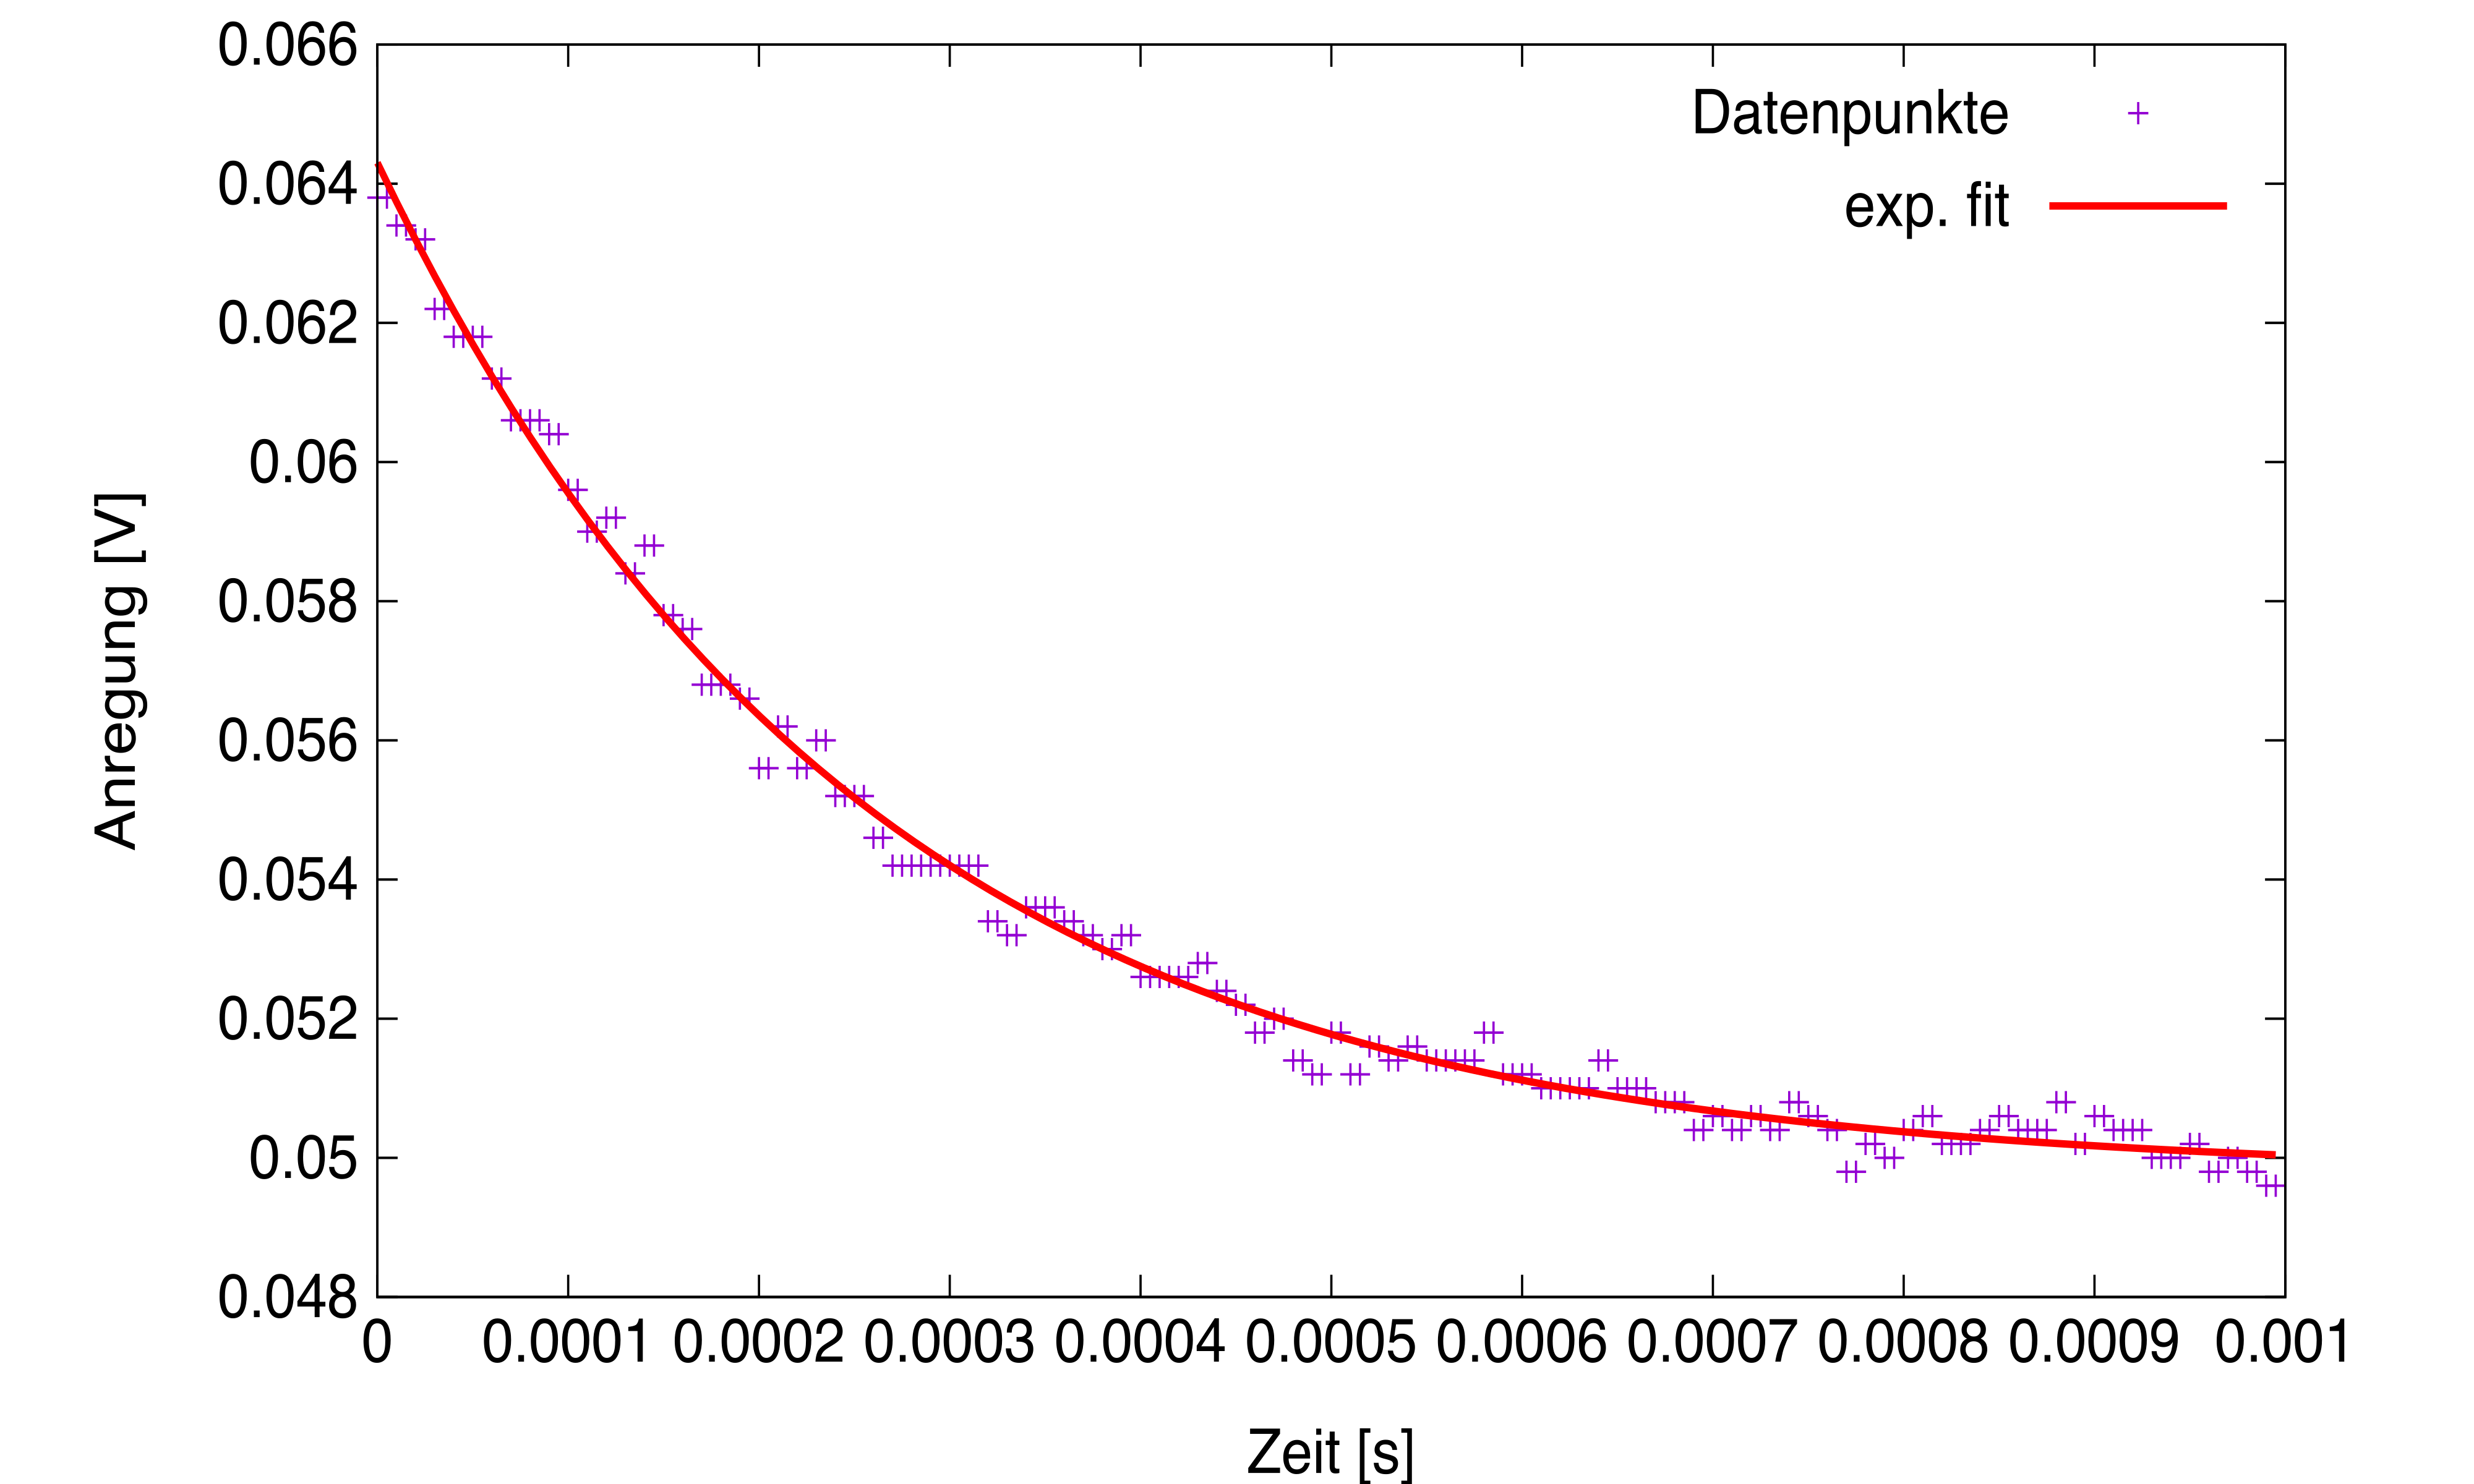
\includegraphics[width=11cm]{../../Bilddateien/2/spontane_emission_data_t_expfit.png}
    %%     \caption{Die gemessene Spannung als Funktion der Zeit mit exponentieller Kurvenanpassung.}
    %%     \label{fig:2:spontaneEmissionDataTExpFit}
    %% \end{figure}
    %% ======================== 

    \begin{table}[H]
        \centering
        \begin{tabular}{c|cc|cc|cc}
            \hline
             & $a$ in $\si{\volt}$ & $u(a)$ in $\si{\volt}$ & $\tau$ in $\si{\s}$ & $u(\tau)$ in $\si{\s}$ & $c$ in $\si{\volt}$ & $u(c)$ in $\si{\volt}$ \\
            \hline\hline
            $f_{a,\tau,c}$ & $0.015$ & $8.1\cdot 10^{-5}$ & $0.00025$ & $3.6\cdot 10^{-6}$ & $0.05$ & $5.18\cdot 10^{-5}$ \\
            \hline
        \end{tabular}
        \caption{Die Parameter der exponentiellen Kurvenanpassung.}
        \label{tab:2-spontaneEmissionDataTExpFit}
    \end{table}
    Der $RSS$ Wert dieser exponentiellen Kurvenanpassung liegt bei $RSS(f_{a,\tau,c}) = 1.63014\cdot 10^{-5}$.

\end{document}